\pdfinfo{%
  /Title    ()
  /Author   ()
  /Creator  ()
  /Producer ()
  /Subject  ()
  /Keywords ()
}

\section{Benutzerprofile löschen}
\subsection{Schnellauswahl der Profile}
Hat man den Menüpunkt ``Profile löschen'' ausgewählt, kommt man auf eine Seite, auf der man durch auswählen von Anfangsbuchstaben sich die Benutzer anzeigen lassen kann. Der ausgewählte Buchstabe gilt dabei nur 
als Anfangsbuchstabe für die Benutzer.\\
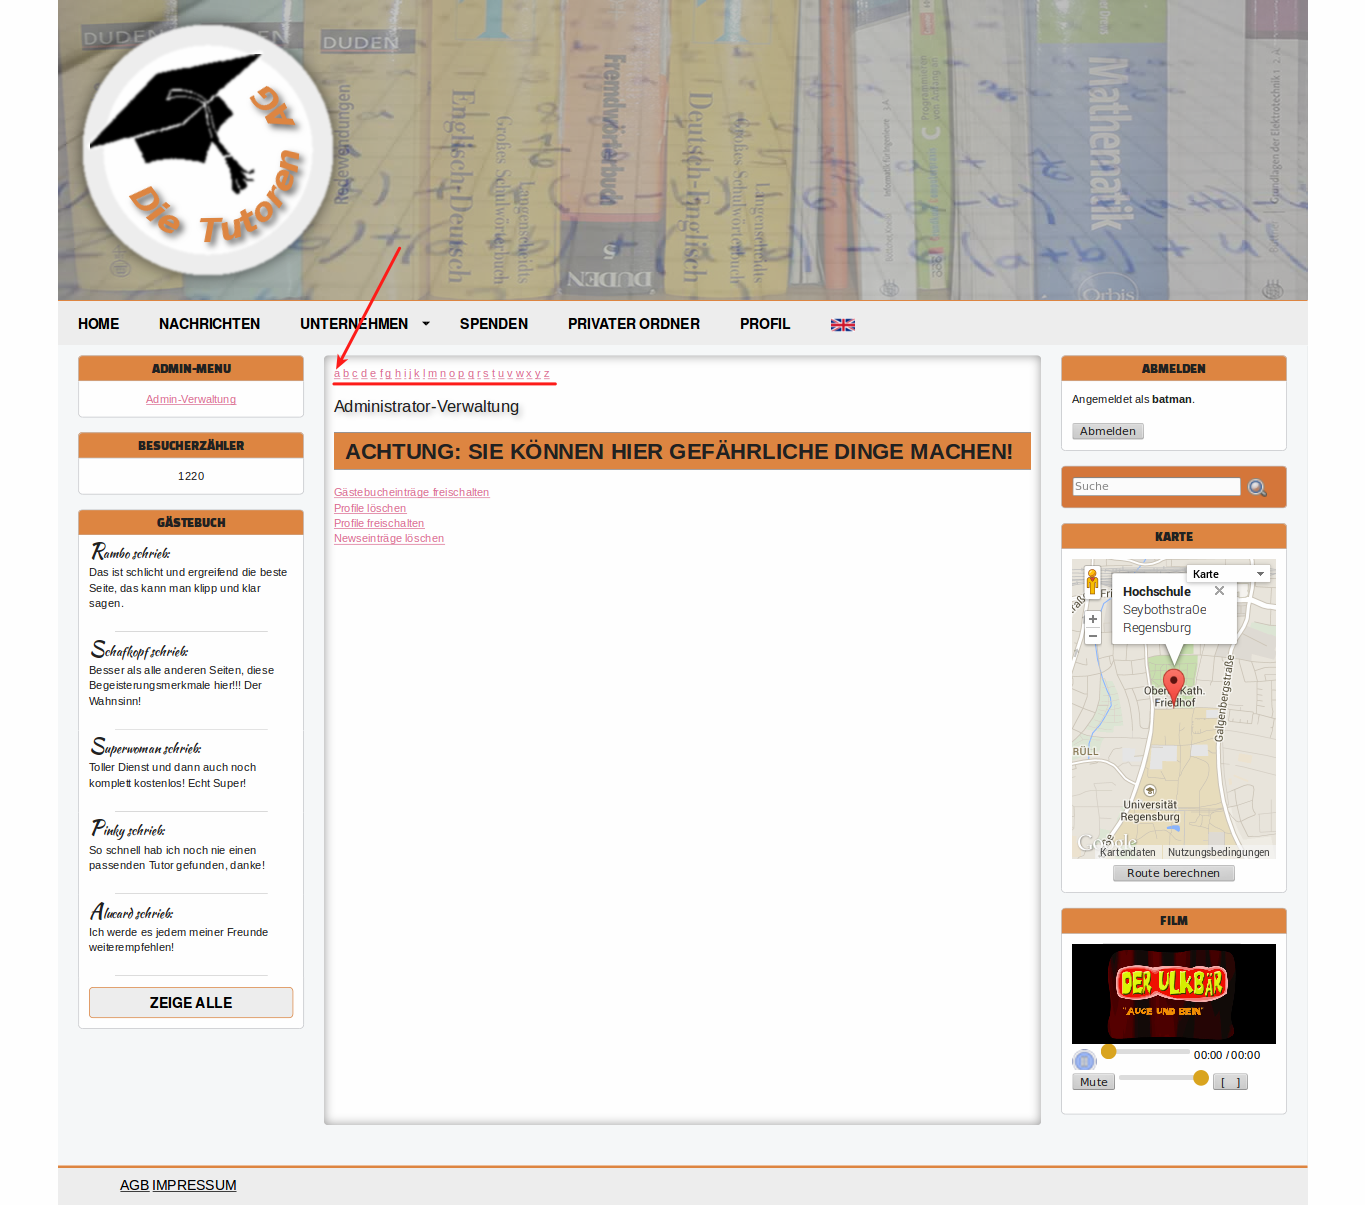
\includegraphics[width=1\textwidth]{../Screenshots/de/admin/admin_delprofile_select}
\newpage
\subsection{Profilübersicht und löschen von Profilen}
Hat man die gewünschten Benutzer ausgewählt, erscheinen diese als Tabelle aufgelistet.
Durch klicken auf den Benutzernamen wird man zu seinem Profil weitergeleitet, sodass man sich das Profil anschauen kann. In der rechten Hälfte der Tabelle kann man durch klicken auf die Checkboxen den User vormerken
zum löschen, durch die Auswahl ``Absenden'' kann man die ausgewählten Benutzer wirklich löschen. Durch ``Zurücksetzen'' setzt man die Auswahl zurück. Die Buchstabenauswahl ist weiterhin sichtbar, genauso wie die 
Schnellauswahl für das Admin-Interface.\\
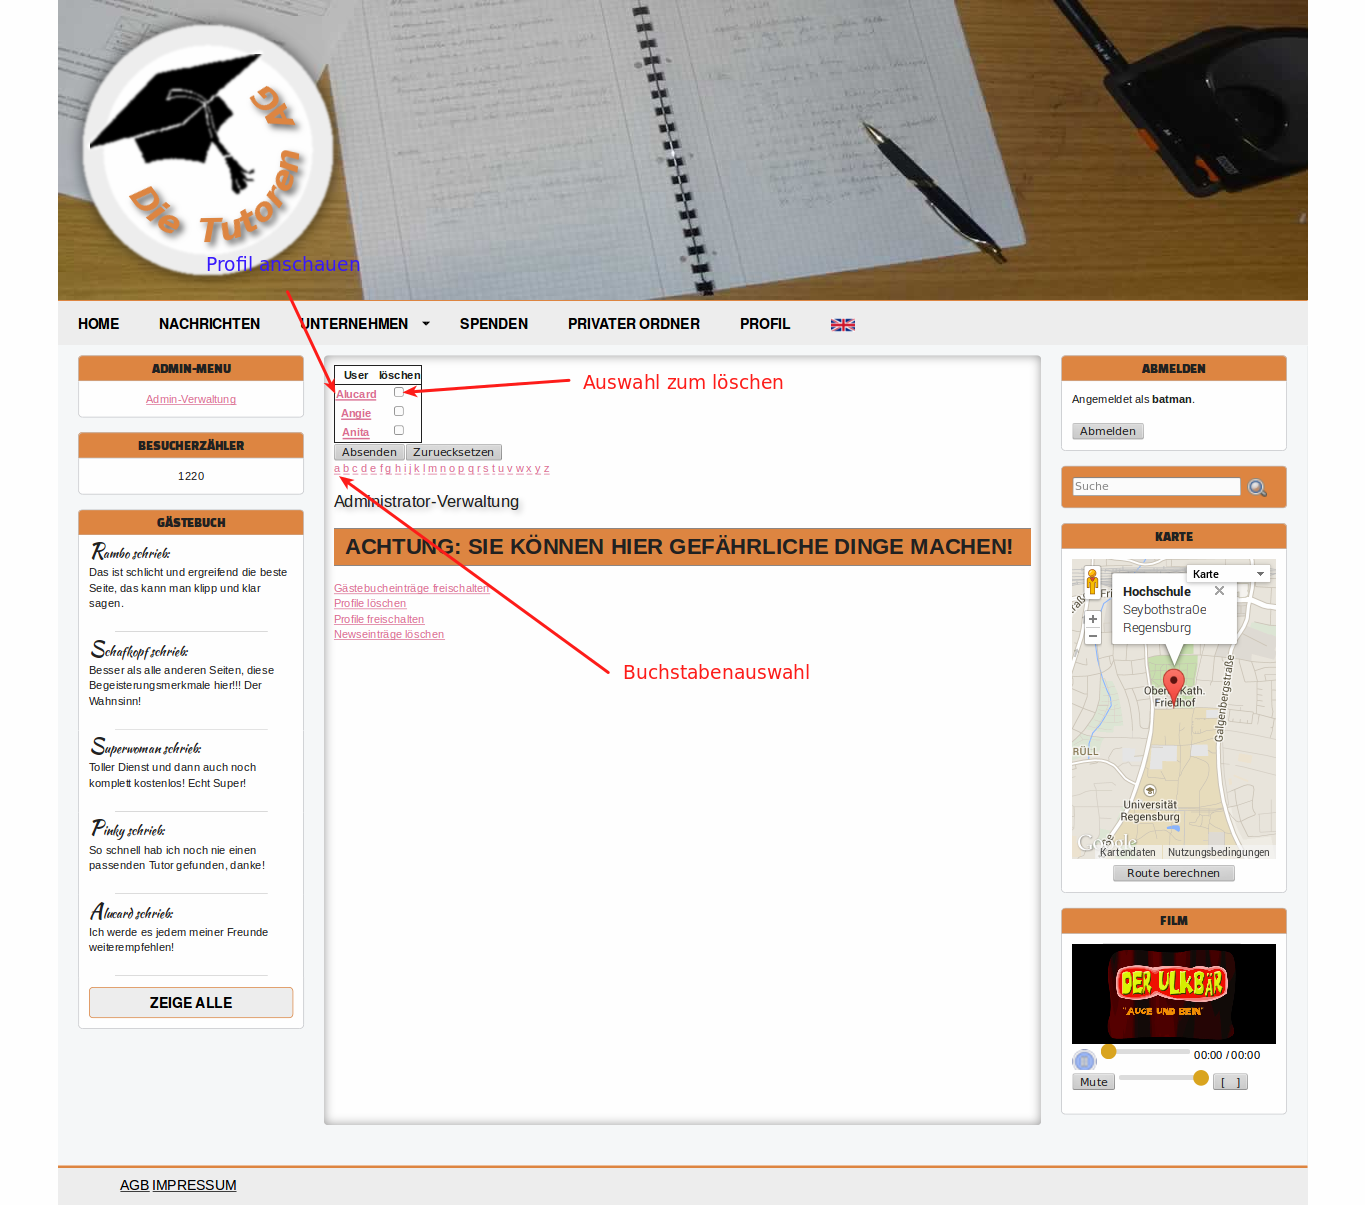
\includegraphics[width=1\textwidth]{../Screenshots/de/admin/admin_delprofile_del}